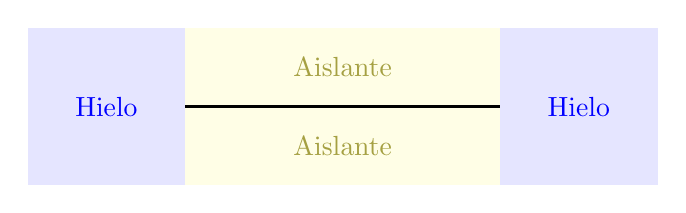
\begin{tikzpicture}
\pgfmathsetmacro{\len}{6}
\fill[blue!10!white] (0,0) rectangle (2,2);
\fill[blue!10!white] (\len,0) rectangle ({\len + 2},2);
\node[blue] at (1,1) {Hielo};
\node[blue] at (1 + \len,1) {Hielo};

\fill[yellow!10!white] (2,0) rectangle ({\len}, 2);

\node[yellow!60!black] at ({1 + \len / 2}, 1.5) {Aislante};
\node[yellow!60!black] at ({1 + \len / 2}, 0.5) {Aislante};

\draw[very thick, black] (2,1) -- (\len, 1);
\end{tikzpicture}
